%%%%%%%%%%%%%%%%%%%%%%%%%%%%%%%%%%%%%%%%%%%
%	PREAMBLE
%%%%%%%%%%%%%%%%%%%%%%%%%%%%%%%%%%%%%%%%%%%
\documentclass[12pt]{report}	
\usepackage[letterpaper, margin=1.25in]{geometry}
\usepackage[titletoc]{appendix}
\usepackage{fancyhdr}
\usepackage{titlesec}
\usepackage{float}
\usepackage{tocloft}
\usepackage{chngcntr}
\usepackage[nottoc,notlof,notlot]{tocbibind}
\usepackage{hyperref} % for URLs
\usepackage{graphicx} % for inserting images
\usepackage[all,defaultlines=3]{nowidow}
\usepackage{listings}
\usepackage[super]{nth}

%------------------------------------------
% 	MISC SETTINGS
%------------------------------------------
% configuration for "listings" package
\lstset{
	breaklines=true,
	basicstyle=\small,
	frame=single,
}

\newcommand{\inlineCode}{\lstinline[basicstyle=\footnotesize\ttfamily]}
%------------------------------------------
% 	PAGE STYLE SETTINGS
%------------------------------------------
\pagestyle{fancy}
\normalfont

% Remove word "Chapter" from chapter titles
\titleformat{\chapter}{\normalfont\huge}{\thechapter.}{20pt}{\huge\it}

% --- Headers and Footers ---
% Set up command to format chapter headers ("1. Chapter Name")
\newcommand{\chapterheaders}{
	\fancyhead[R]{
		% Only display chapter numbers greater than 0
		\ifnum\value{chapter}>0 \thechapter. \fi
		\MakeUppercase{\leftmark}
	}
}
% Set up a command to format References headers ("References")
\newcommand{\referenceheaders}{
	\fancyhead[R]{
		% Don't display the chapter number
		\leftmark
	}	
}

% Set the default header options
\setlength{\headheight}{15pt}
\fancyhf{}
\chapterheaders

% Add page number to footer
\fancyfoot[C]{\thepage}
\renewcommand\chaptermark[1]{\markboth{#1}{}}

% Set up a command for custom appendix page numbering
\newcommand{\appendixpagenumbering}{
	\break
	\pagenumbering{arabic}
	\renewcommand{\thepage}{\thechapter-\arabic{page}}
}

%------------------------------------------
% 	TABLE OF CONTENTS SETTINGS
%------------------------------------------
\renewcommand{\cftchapaftersnum}{:\space}
\newlength{\mytoclen}
\settowidth{\mytoclen}{\cftchapaftersnum}
\setlength{\cftchapnumwidth}{\dimexpr\mytoclen+1.5em}

%------------------------------------------
% 	FIGURE, TABLE, AND EQUATION SETTINGS
%------------------------------------------
% Put thin border around all figures and tables
\floatstyle{boxed}
\restylefloat{figure}

% Change the default figure/table/equation numbering conventions
\counterwithout{figure}{chapter}
\counterwithout{table}{chapter}
\counterwithout{equation}{section}

% Change the spacing of the Lists of Figures/Tables to accommodate prefixes
\renewcommand{\cftfigpresnum}{Figure\ }
\renewcommand{\cfttabpresnum}{Table\ }
\renewcommand{\cftfigaftersnum}{:\space}
\renewcommand{\cfttabaftersnum}{:\space}
\newlength{\mylen}
\settowidth{\mylen}{\cftfigpresnum}
\setlength{\cftfignumwidth}{\dimexpr\mylen+4.5em}
\setlength{\cfttabnumwidth}{\dimexpr\mylen+4.5em}
%\renewcommand{\cftfigfont}{Figure }	% Alternative fix for 
%\renewcommand{\cfttabfont}{Table }		%	adding prefixes

% Set up a command for custom appendix figure/table numbering
\newcommand{\appendixfigurenumbering}{
		\renewcommand{\thefigure}{\thechapter-\arabic{figure}}
		\renewcommand{\thetable}{\thechapter-\arabic{table}}
		\setcounter{figure}{0}
		\setcounter{table}{0}
}

% Redefine figure caption convention
\renewcommand{\figurename}{FIGURE}
\renewcommand{\tablename}{TABLE}

%------------------------------------------
% 	REFERENCE SETTINGS
%------------------------------------------
\renewcommand{\bibname}{References}
\bibliographystyle{apalike}

% remove label from references, but preserve hanging indent
\makeatletter
\setlength\bibindent{2.5em}
\renewcommand\@openbib@code{%
   \leftmargin\bibindent
  \itemindent -\bibindent
  \listparindent \parindent
  \parsep \z@
  \labelsep0pt
}
\renewcommand\@biblabel[1]{}
\makeatother

%%%%%%%%%%%%%%%%%%%%%%%%%%%%%%%%%%%%%%%%%%%
%	FRONT MATTER
%%%%%%%%%%%%%%%%%%%%%%%%%%%%%%%%%%%%%%%%%%%
\begin{document}	
\pagenumbering{roman}

%------------------------------------------
%	TITLE PAGE
%------------------------------------------
\title{\large{Carleton University \\
	COMP 4905 - Honours Project
	} \\
	\LARGE{\bf RT-Tuner:\\A real-time audio analysis tool}}
\author{Justin W. Hoggart \\
	\\\emph{Supervisor}: \\
	Louis D. Nel, Ph.D.,\\
	School of Computer Science}
\date{\today}

\maketitle
\clearpage

%------------------------------------------
%	ABSTRACT
%------------------------------------------
\begin{abstract}
	\thispagestyle{plain} %to add page number to abstract
	The RT-Tuner application is a real-time audio analysis tool whose purpose is to first acquire information about an audio signal, and then use this information to help a user in tuning their musical instrument in a user-friendly manner. This task is accomplished by recording a live audio feed, processing the data obtained in this recording in order to obtain the fundamental frequency underlying the audio signal, and then converting this frequency value into a visual representation of the pitch based on the 12-tone chromatic scale. Topics examined in this paper include fundamental music theory; sound visualization techniques; the basics of digital signals processing, including filtering, windowing, and the Fourier transform; and pitch estimation techniques. The combined process of applying a Hanning window, a low-pass filter, and the fast Fourier transform to a raw audio signal, and then performing harmonic product spectrum analysis appears to be a reasonably effective method of estimating pitch within a range of $\sim100~Hz$--$330~Hz$.
\end{abstract}
\clearpage

%------------------------------------------
%	ACKNOWLEDGEMENTS
%------------------------------------------
\chapter*{Acknowledgments}
\setcounter{page}{2} % to accommodate adding pagenumber to abstract

\indent I owe a good deal of gratitude to Professor Louis D. Nel for agreeing to supervise me in this project, and for providing the valuable advice that I needed in order to find my way toward what turned out to be a very interesting topic. I would also like to express my appreciation to a number of researchers and software developers without whose works this project would have proven to be an insurmountable task for me: Matteo Frigo of the IBM Austin Research Laboratory and Steven G. Johnson of the Massachusetts Institute of Technology for their work on ``FFTW3: The Fastest Fourier Transform in the West''; Gary P. Scavone of McGill University for his work on the ``RtAudio'' audio input/output API; the many and varied contributors to the ``wxWidgets'' cross-platform GUI library, who are unfortunately left unidentified to me; Davide Rondini, David Schalig, Jose Luis Blanco, and Val Greene for their work on the ``wxMathPlot'' graphing tool; and Marco Cavallini for his ``Koan wxIndustrialControls'' package. I'd also like to offer my thanks to Bjorn Roche whose blog ``BJORG'' proved extremely helpful in allowing me to wrap my mind around a number of the subtleties involved in the audio analysis process that I would have otherwise struggled with.
\clearpage

%------------------------------------------
%	TABLE OF CONTENTS
%------------------------------------------
\tableofcontents
\clearpage

%------------------------------------------
%	LISTS OF FIGURES AND TABLES
%------------------------------------------
\listoffigures
%\listoftables
\clearpage

%%%%%%%%%%%%%%%%%%%%%%%%%%%%%%%%%%%%%%%%%%%
%	MAIN MATTER
%%%%%%%%%%%%%%%%%%%%%%%%%%%%%%%%%%%%%%%%%%%
\pagenumbering{arabic}

% ___ Chapter 1 - Introduction ___
\chapter{Introduction}
\indent This project was intended to devise a piece of software to allow for the examination and analysis of real-time audio data, with the end goal of developing a user-friendly graphical tool that could allow a user to track and adjust their musical instrument's tuning in real-time. The high-level approach to this was to start by developing a core application to capture an audio signal and parse out useful data from it, and then to make use of that core and the information it gathers to make a decision regarding the audio signal, specifically to decide which musical note the audio signal most closely resembles. Beginning with very little knowledge of or experience with either musical theory or digital signals processing, a great deal of basic research was required to establish a suitable foundation of knowledge, and then build upon it. The report which follows, therefore, will cover in some detail fundamental topics such as basic music theory, sound visualization techniques, and fundamental digital signals processing concepts, while also delving a bit more deeply into more complicated subjects like frequency spectrum analysis, signal filtering and windowing, and the relationships between time and frequency, and frequency and musical pitch. 

\indent In addition to the above-mentioned theory topics studied for this project, a number of unfamiliar software packages needed to be learned, including an audio input/output API package, a large graphical user interface package, and a fairly complex mathematical library, and their inherent learning curves certainly added to the challenge. Since these concerns had such a profound effect on the development process, some time will be spent examining these and other particular implementation details, including the configuration of the development environment and the code itself. Additionally, a sort of guide will be provided concerning how this application might most easily be re-purposed or appended to in the future, and how the existing code might most easily be modified and interfaced with.

\indent Finally, an examination of the end result of this project will be performed, discussing things that worked, things that did not, and evaluating various design decisions that were made, and how things might have been improved. As part of this, some suggestions for future improvements or additions, or different approaches that might be worth considering will be provided. With this outline in mind, let's begin with a look at some necessary fundamentals.
\clearpage


% ___ Chapter 2 - Overview: From Audio Signal to Visual Representation ___
\chapter[Fundamentals: From Audio Signal to Visual Representation]{Fundamentals: From Audio Signal \\to Visual Representation}

% --- Section 2.1 - Capturing Audio Data ---
\section{Capturing Audio Data}	
\indent In order to move from our starting point of vibrations in the air to the end point of a visual representation of the musical note being played, we first need to convert the audio signal from its analog representation into a digital one that the computer can work with. The easiest path to accomplishing this is to use a microphone to capture the vibrations and convert them into a raw digital pulse-code modulation (PCM) signal, which can then be interpreted using an audio input/output software library. A number of such software packages were considered for this project, including the \emph{libsndfile} package\footnote{\url{http://www.mega-nerd.com/libsndfile/}}, the \emph{PortAudio} package\footnote{\url{http://www.portaudio.com/}}, and the \emph{RtAudio} package\footnote{\url{http://www.music.mcgill.ca/~gary/rtaudio/}}, all of which provide an application programming interface (API) for interacting with audio data. Although very interesting, the \emph{libsndfile} package was eliminated from consideration, as it was designed for use in a Linux environment on pre-recorded audio data, rather than the Windows-based real-time application that we want. And although both \emph{PortAudio} and \emph{RtAudio} are very similar in their capabilities, \emph{RtAudio} was ultimately selected simply because, as it was developed in the C++ language, it was an easier process to interface this with the rest of the code for this project than the C-based interface that \emph{PortAudio} provided.

\indent Having decided on an audio integration API, the next step is to use this package to incorporate the audio data into the program, allowing us to manipulate and analyze the signal. For \emph{RtAudio} in particular, this requires following a fairly simple procedure. First, we establish a connection to the computer system's input device (i.e. the microphone) and open a recording stream, passing parameters telling the input device, for example, what format to convert the audio signal into as it records, what sample rate to use while doing so, and the number of frames to capture at a time. Along with these settings for the input device, we also need to pass the name of a callback function which will be called every time the input device returns with the requested data, and whose purpose it will be to process this information. We then issue a command to start capturing this audio stream, which will continue to run until manually stopped, or until the program is terminated.

\indent Some important terminology was introduced in the previous paragraph, so let's take a moment to clearly define these terms. The recording {\bf stream} is simply a sort of pathway for the continuous flow of the audio data that we are capturing, which guides this data from the microphone to the program. The {\bf data format} describes the digital representation of the data that is captured, ultimately taking the form of a number, for example an unsigned integer, or a floating point number; for this application we are using a 64-bit (or ``double precision'') floating point number. The {\bf sample rate} of an audio signal is the number of samples of audio captured by the stream per second, measured in Hertz (Hz)~\cite{Audacity-nd}, where a ``sample'' is a sort of snapshot of the audio at a given moment in time; since we are interested in real-time processing with this application, a relatively small sample rate of 8 kHz is used here to ease the processing overhead. And finally, the {\bf frame rate} is the number of sample frames to consider at a time, where a ``frame'' is a set of samples that are coincident in time~\cite{Bernard2001}; a relatively large frame rate of 4096 is used here in the interest of increasing the data points that we receive, and thus the accuracy of the frequency resolution (this will be discussed further in a later chapter). With all of this in mind and our audio signal being captured, we must now turn to the question of exactly what it is that we are looking for in this signal.


% --- Section 2.2 - Music Theory Basics ---
\section{Music Theory Basics}
\indent The stated goal for this project is to aid a user in ``tuning'' their instrument -- so what exactly does this mean, musically speaking? Well, tuning an instrument consists of configuring the instrument's moving parts (increasing or decreasing the tension in guitar strings, for instance) so that they consistently produce a specific note, or notes. This means that we will need to parse the raw audio signal that we discussed in the previous section in order to determine whether the sound matches the desired musical note. But before we can look to the task of interpreting the signal in the terms of musical notes, we first need to look at what a musical note really is; to this end, let's take a brief look at some basics of musical theory. It is fairly common knowledge that notes are the fundamental building blocks of musical performance, and the language with which we communicate the specifics of musical sounds to each other. In that vein, the following sequence should seem familiar~\cite{SeventhString-nd}: 
$$ A_4 B\flat_4 B_4 C_5 C\sharp_5 D_5 E\flat_5 E_5 F_5 F\sharp_5 G_5 G\sharp_5 $$

\indent This is one of the most common representations of musical notes, that of the 12-tone chromatic scale, with notes being represented in the form of a letter from A to G (indicating the ``pitch class'' of the note), a number from 0 to 8 (representing the ``octave''), and occasionally a $\flat$ (flat) or $\sharp$ (sharp) symbol to indicate a half-step difference in pitch. At its most basic level, a note is a pitched sound, where pitch is a perceptual property related to the frequency of the sound; note that the perception-dependent nature of pitch makes it more of a subjective, psycho-acoustical characteristic~\cite[p.145]{Hartmann1997} -- that is to say, it's more in the domain of psychology than the strict, objective domain of pure physics. Despite this, however, we can still fairly accurately quantify this phenomenon in terms of the sound's ``frequency'', such as by using techniques to determine the overall ``fundamental frequency'' of the sound.

\indent Let's look at some of these properties in slightly more detail. It should seem fairly obvious that the seven different letters mentioned above are insufficient to represent every possible note on their own -- but they don't have to, because the psycho-acoustical nature of pitch has the extraordinary effect of making notes seem very similar to each other over a consistent, recurrent period~\cite[p.776]{Randel2003}. Particularly, we perceive pitch logarithmically~\cite{Hass2003} with respect to frequency, meaning that any two notes whose fundamental frequencies are in a ratio equal to any power of two seem to be very similar to each other, which is where the term {\bf pitch class} comes from -- two notes whose fundamental frequencies are not the same, but who nevertheless sound alike are said to be in the same pitch class (the notes at 55Hz and 440Hz are both classified as ``A'' notes, for example). The periodic nature of these classifications is also where the {\bf octaves} come in. The octave number accompanying the note class lets us identify exactly where in this cycle a note is in comparison to any other: we can clearly see that the note $A_1$ is a much lower frequency than $A_4$ (55Hz and 440Hz, respectively), and that $F\sharp_4$ is a slightly higher frequency than $B_3$ (370Hz and 246.9Hz) simply by comparing their octaves. Noting that there are exactly 12 half-steps between each corresponding note from one octave to the next (i.e. between $A_3$ and $A_4$), and choosing a known anchor point (commonly ``A440'', which is $A_4$ at 440Hz), we can find the precise frequency of a given note using the following formula~\cite{Qehn-nd}: 
$$ F = (2^\frac{1}{12})^n \times 440 \mbox{ Hz} $$

\indent Where $F$ is the pitch frequency, and $n$ is the number of half-steps away from the known frequency ($A_4$) that the note is. (Note also that we can use this formula in the other direction, solving for the number of half-steps away from the anchor when we have the frequency.) Now, this is all well and good when a sound happens to exactly match one of these fundamental frequencies, but what if it's off slightly? This brings us to the concept of the ``cent''. Since we know that there are 12 half-steps in a given octave, and each half-step is some constant distance apart from one another, we can fairly easily assign a measure of the distance between two half-steps. A {\bf cent} is one such measure, defined as a logarithmic unit ranging in value from 0 to 100 indicating the distance between two successive half-steps~\cite{Suits-nd}. For example, a sound with a pitch frequency of 450Hz is said to be the note $A_4$ with an offset of 39 cents, meaning that it sounds most like the note $A_4$ (and, indeed, such small variations are often indistinguishable to the naked ear), but is about 39\% of the way between $A_4$ and $B\flat_4$. So now that we know some of these specifics, how do we determine which information is most relevant for our instrument-tuning purposes, and how do we visualize it, graphically?


% --- Section 2.3 - Visualizing Sound ---
\section{Visualizing Sound}
\label{sec:vissnd}
\indent Based on what was discussed in the previous section, it seems clear that the most important information that we can extract from an audio signal is its fundamental frequency. Since what the user is interested in is the tuning of an instrument, to allow them to properly tune their instrument we will obviously need to show them information about how this frequency relates to musical notes. There are two possible approaches that we can take for this: we can ask the user precisely what note they are looking for and compare that to the observed signal, offering a ``yes\slash no'' or ``hot\slash cold'' sort of response; or we can automatically detect information about the note, octave, and offset that corresponds with the fundamental frequency that is found in the observed signal, and then present this data to the user. From an ease of use perspective, the latter is clearly the better option, and it simultaneously allows us to provide the user with more detailed information and more flexibility on what to do with that information, so this is the direction that was followed. With this in mind, let's examine what may be the best ways to get this information across to the user.

\indent We'll get into the details of exactly how to determine fundamental frequency in subsequent chapters, but it should make sense that the first step includes capturing the overall frequency profile, or ``spectrum'', from the audio signal. Since the purpose of this tool is ostensibly to correct the tuning of an instrument, we must assume that the audio signal will not be perfectly aligned with any particular note at the outset, and so allowing the user to see the spectrum could prove useful in guiding them toward their goal. There are two primary methods in which this information is often represented: the first is a spectrogram, which typically takes the form of a three-dimensional graph plotting frequency against time on the X and Y axes, and representing the intensity of a given point in the third dimension, whether via a traditional Z-axis or through use of a colour gradient; the second is a simple two-dimensional graph, usually plotting frequency vs. amplitude, as depicted in Fig.~\ref{fig:spectrum}. Since we are really only interested in the frequencies and their magnitudes we don't want to overload the user with information, and so the simpler two-dimensional approach seemed most appropriate.

\begin{figure}[!ht]
	\centering
	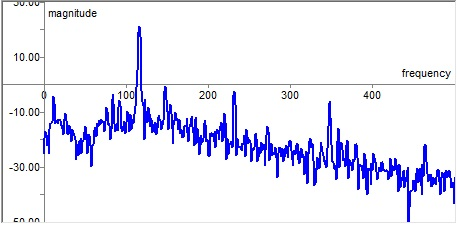
\includegraphics[width=120mm]{spectrum.jpg}
	\caption[Spectrum Graph]{An example of a simple two-dimensional spectrum graph.} 
	\label{fig:spectrum} 
\end{figure}

\indent The other important information to share is the evaluation relating to note, octave, and offset. A simple way to approach this would be to simply display the data in text form, which has the benefit of being unambiguous and easy to understand, but is perhaps a little bit bland. Perhaps a more aesthetically engaging option is to use a needle gauge, which has the twin benefits of being fairly intuitive (since this is the form that most portable guitar and instrument tuners currently take) and allowing a clear visual representation of how near or far from the desired frequency the observed signal is. Or, indeed, since the textual approach can be fairly unobtrusive we could easily combine the two, allowing the user the freedom to circumstantially choose which format they prefer. The textual representation would be a very simple matter as we would necessarily already have all of the measurements and data available, so we could simply display this to the interface; the needle gauge, however, is more complicated. The ideal approach would be to have the gauge dynamically adjust its scale dependent on which fundamental note is closest to the current frequency profile, but since the spectral landscape is likely to be changing almost constantly this would result in a great deal of computational overhead, as we would need to recalculate the bounds for the scale with every sample of audio that we test. And so, despite the diminished usability, this approach was eschewed in favour of the much more simplistic one depicted in Fig.~\ref{fig:gauge}: narrowing the focus to a particular band of frequencies typical with respect to one instrument -- namely the bass guitar. Thus, the scale was fixed to represent the range of relevant fundamental frequencies for this instrument, specifically ranging from just below the note $B_0$ at $\sim30$ Hz, to just above the note $E_4$ at $\sim330$ Hz~\cite{Anon2014a}.

\begin{figure}[!ht]
	\centering
	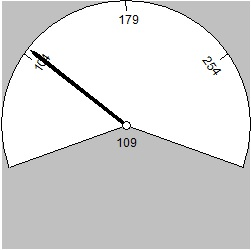
\includegraphics[width=60mm]{needlegauge.jpg}
	\caption[Tuner Needle Gauge]{The needle gauge, indicating the fundamental frequency relative to the 30Hz--330Hz scale.}
	\label{fig:gauge} 
\end{figure}

\indent Having covered the general sort of visual components that were deemed to be necessary, we now turn to the practical details of how these were implemented. First, a general graphical user interface (GUI) development package for C++ was necessary, and this was chosen, frankly, rather arbitrarily; after researching a few options, the \emph{wxWidgets}\footnote{\url{https://www.wxwidgets.org/}} package proved to be both very simple to use and very versatile in terms of its capabilities, with a very shallow learning curve. Having decided on \emph{wxWidgets} as the backbone of the GUI, the next step was to find a UI element appropriate for the two-dimensional frequency spectrum graph, and for this the simple-but-effective \emph{wxMathPlot}\footnote{\url{http://wxmathplot.sourceforge.net/index.shtml}} extension package was chosen. Using \emph{wxMathPlot}'s ``mpFXYVector'' object, it's a very simple matter of performing our calculations on each audio sample, generating the X- and Y-vectors (frequency and magnitude, respectively), and telling the program to render them atop the main graph plot. For the textual note-based information, a simple text label was used, with the calculated pitch class, octave, and offset (in cents) indicated plainly. Finally, for the needle gauge the ``AngularMeter'' object was used from a package called \emph{Koan wxIndustrialControls}\footnote{\url{http://wxcode.sourceforge.net/showcomp.php?name=kwxIndustrialIndicators}}, whose needle points at the current fundamental frequency relative to the scale discussed earlier. With these graphical elements in place, it's time that we looked at converting the raw audio data into the frequency and note information that we want to display.


% ___ Chapter 3 - Audio Post-Processing ___
\chapter{Audio Post-Processing}
% --- Section 3.1 - Time Domain vs Frequency Domain ---
\section{Time Domain vs Frequency Domain}
\indent With most of the aesthetic and design decisions laid out, it's now time to take a look at the more technical details of precisely how to manipulate the raw audio data in order to acquire the results that we need. To that end, there are a number of concepts and techniques related to digital signals processing (DSP) and spectrum analysis that will be discussed in this chapter, including filters, windowing functions, the Fourier transform, and an exploration of pitch estimation techniques. However, before we dive into these there's one important basic aspect that needs to be understood, namely the relationship between time and frequency. 

\indent In order to capture the audio signal from the air, a microphone measures the vibrations as they are detected, resulting in data that is a function of the amplitude of the sound waves against the passage of time. This time domain data allows us to see the general shape of the signal over a particular time interval, which can be valuable, but it doesn't quite give us the whole story. The frequency domain allows us to see another side to the data, eschewing time in favour of revealing the frequency profile underlying the particular snippet of audio in question, which can help us to determine why a signal behaves as it does. Take Fig.~\ref{fig:tvf1}, for example:

\begin{figure}[h]
	\centering
	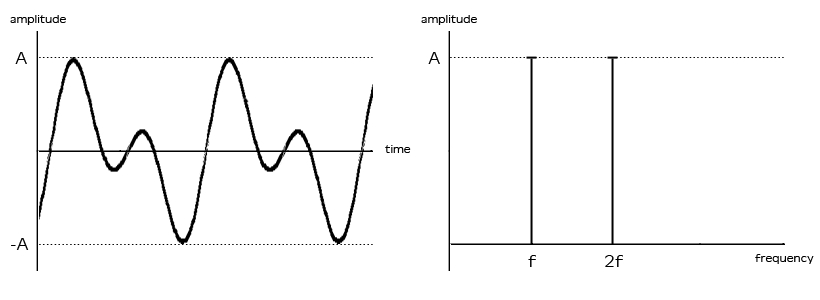
\includegraphics[width=120mm]{timevfreq-02.jpg}
	\\ \emph{A relatively simple union of two sine functions.}
	\caption[Time vs. Frequency: Clean]{Time domain (left) vs. frequency domain (right)~\cite{Anon2014b}.} 
	\label{fig:tvf1} 
\end{figure}	

\indent We can see from the time domain data on the left that the sound repeats periodically, and has a sort of ``hitch'' in it evidenced by the slight dip in the amplitude in the second portion of each repeating section, which is very useful to see since our ears may not necessarily catch a subtle change like this. However, there's no clear indication for exactly \emph{why} this hitch occurs. Looking at the frequency domain data on the right, though, makes things clearer: there are two distinct frequencies interacting with each other, causing an interference pattern which results in the behaviour that we are seeing. This is especially valuable when dealing with a real-world signal, which is never as clean as the two sine signals depicted in Fig.~\ref{fig:tvf1}. Looking at a much messier example, Fig.~\ref{fig:tvf2} shows a time domain representation that is very difficult to decipher, with the signal appearing very erratic, but when shown side-by-side with the corresponding frequency data we can see which prominent frequency ranges the signal is a product of, and how weak or strong they are relative to each other. 

\begin{figure}[h]
	\centering
	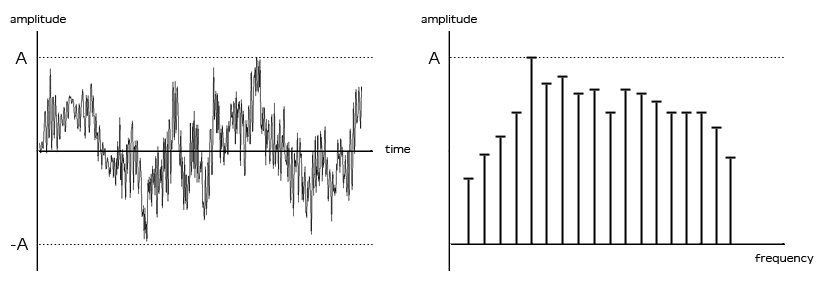
\includegraphics[width=120mm]{timevfreq-03.jpg}
	\\ \emph{A much messier signal with many different frequency interactions.}
	\caption[Time vs. Frequency: Messy]{Time domain (left) vs. frequency domain (right)~\cite{Anon2014c}.} 
	\label{fig:tvf2} 
\end{figure}	

\indent Generally, when dealing with audio post-processing one will wish to utilize the data in both the time and frequency domains in order to get a clear picture of what's happening, and to manipulate and mould the signal to achieve whatever ends are desired, and this particular application is no different. Although it may seem that we only need the frequency-domain data, since we are ostensibly ``only'' looking for the fundamental frequency, some manipulation in the time domain is essential for preparing the signal in such a way as to make analysis of the frequency data simpler and more reliable, which is where filters and windowing functions come into play.
\clearpage

% --- Section 3.2 - Filters and Windowing Functions ---
\section{Filters and Windowing Functions}
\subsection*{Filters}
\indent The basic concept of a filter should be very familiar, whether we're talking about coffee makers or audio processors: a filter is something which, when applied to some sort of flow, allows some things to pass through and not others. For an audio stream, depending on the frequency data that the audio signal contains and what one is trying to do with it, a variety of filters can be used to help eliminate potentially problematic data, while keeping the remainder intact. For instance, most sounds generated by musical instruments contain such a wide range of frequencies all at once that determining which of these frequencies is the fundamental can be very difficult, especially when taking into account the existence of harmonics\footnote{Without going into too much detail, it suffices to know that a harmonic is a component frequency of a signal which is a multiple of the fundamental frequency~\cite{Chisholm1911}.}. In order to try to minimize the chances of a false positive with respect to the fundamental note, we can filter the signal, limiting our data to the frequency range that we are concerned with (called the {\bf passband}) and stopping some of the extraneous frequencies (called the {\bf stopband}), thus eliminating some of the potentially confusing interactions these could cause. In our case, since the focus for this project has been narrowed to the fundamental frequencies of a standard bass guitar, we can use what is called a {\bf low-pass filter} which is used to block the frequencies higher than some threshold (here we use 330 Hz as a cutoff, which is just above the fundamental frequency for the highest expected note, $E_4$), and allow all other frequencies to pass through largely untouched~\cite[p.201]{Park2009}.

\indent The low-band filter that was used in this instance was a {\bf biquad} (so called because the equation describing it contains two quadratics)~\cite{Roche2012b}, which is a second-order digital filter that affords a greater degree of control over which portions of the signal are filtered than would a simpler first-order filter. In order to use this filter, one first needs to determine a number of parameters, first and foremost of which are the sample rate of the audio as it passes through the filter, $F_s$, and the so-called {\bf centre frequency}, $f_0$, which is the ``significant'' frequency for the filter (whatever that may mean, in the context of a given application). It's important to note that the centre frequency needs to be less than or equal to the Nyquist frequency (defined as one-half the sampling rate, $\frac{F_s}{2}$~\cite[p.201]{Park2009}) in order to prevent the signal from exhibiting problematic imperfections, a phenomenon called ``aliasing''~\cite{Zawistowski-nd}. The next preliminary step is to calculate some intermediate values: $w_0 = 2 \pi \times \frac{f_0}{F_s}$, $c = \cos(w_0)$, $s = \sin(w_0)$, and $\alpha = \frac{s}{2 \sqrt{2}}$~\cite{BristowJohnson-nd}. With these values in-hand, we then calculate the final coefficients for the filter:
\clearpage
$$a_0 = 1 + \alpha \quad\quad\quad\quad b_0 = \frac{1 - c}{2}$$
$$a_1 = -2 \times c \quad\quad\quad\quad b_1 = 1 - c$$
$$a_2 = 1 - \alpha \quad\quad\quad\quad b_2 = \frac{1 - c}{2}$$

\indent With all of this preliminary legwork taken care of, all that's left is to combine these pieces into the final filter calculation (see Eqn.~(\ref{eqn:lowpass}) below~\cite{BristowJohnson-nd}), which will be applied to each sample in order to achieve the desired effect. (Typically, we want to normalize the coefficients such that $a_0 = 1$ by dividing them by the $a_0$ term to simplify things; below this is done in the filtering equation itself, but it's often prudent to perform this normalization at the coefficient stage, in order to ease computational overhead). Notice that this final filter equation involves a recursive reference to the previous $y$ value ($y_{n-1}$), meaning that each result is dependent on the previous; this has a number of implications, which are largely outside the scope of this project, but it's something to keep in mind\footnote{Take a look at Bjorn Roche's ``Basic Audio EQs'' blog post on the subject for more detail~\cite{Roche2012b}.}.
\begin{equation} 
	\label{eqn:lowpass}
	y_n = [(\frac{b_0}{a_0}) \times x_n] + [(\frac{b_1}{a_0}) \times x_{n-1}] + [(\frac{b_2}{a_0}) \times x_{n-2}] - [(\frac{a_1}{a_0}) \times y_{n-1}] - [(\frac{a_2}{a_0}) \times y_{n-2}]
\end{equation}

\indent Once this filter is applied, we are left with a more concise sample of data to work with, but there are still some potentially problematic aspects that remain which we will need to take care of before passing the signal through the Fourier transform, which brings us to the windowing function.

\subsection*{Windowing Functions}
\indent The Fourier transform will be discussed in more detail in the next chapter, but it's important to be aware of one characteristic of it before we proceed in looking at windowing functions. Namely, the Fourier transform algorithm assumes that the signal that is being provided to it is periodic in nature -- that is to say, that the signal repeats itself over some time span -- but real-world audio signals are almost always non-periodic. This inconsistency between what the Fourier algorithm expects and what the real-world signal actually provides can lead to {\bf spectral leakage}, which are errors that could cause the resulting frequency numbers to be distributed incorrectly, or even ``[create] artifacts at frequencies that aren't actually present in your signal''~\cite{Roche2012a}. So how can we manage this discrepancy?

\indent In order to control for the incompatibility between the ideal and real, we can use a technique called {\bf windowing}, which consists of multiplying the real-world signal by some function with the intent of minimizing spectral leakage, and getting a clearer picture of the true characteristics of the signal. Since one cannot possibly measure an infinitely long signal, every audio signal has a {\bf rectangular window function} applied to it by default, where the rectangular function is simply a multiplication of the signal by one ($w(n) = 1$), with truncated ends making it appear as if the signal suddenly starts and stops. While this can be sufficient in some cases, it is often difficult to parse out relevant detail with much certainty, and all of the initial spectral leakage remains present, so a variety of different windowing functions have been developed tailored to particular needs. Among the most commonly used of these functions is a class referred to as ``Generalized Hamming windows'', which make use of a specialized form of cosine function to taper a signal in the interest of causing peaks to more readily distinguish themselves. Although there are quite a large number of such functions, the relatively simple needs of this project necessitate only a very simple one, and so the {\bf Hann window} was chosen, as it is among the simplest and most widely recognized for being effective at isolating the information that is necessary for our purposes. The Hann window as defined by the formula $w(n) = 0.5 \times (1 - cos(\frac{2 \pi n}{N - 1}))$\footnote{\url{https://en.wikipedia.org/wiki/Hann_function}} creates a smooth, gradual incline/decline from the edges of the signal towards the center, as visualized in Fig.~\ref{fig:hann} below, in contrast to the abrupt changes present at the edges of a rectangular-windowed signal. Because of this prioritization towards the ``center'', applying this function to our initial signal can reduce much of the noise bleeding over between frequency measurements, allowing us to more easily identify the significant frequency ranges contained within.

\begin{figure}[h]
	\centering
	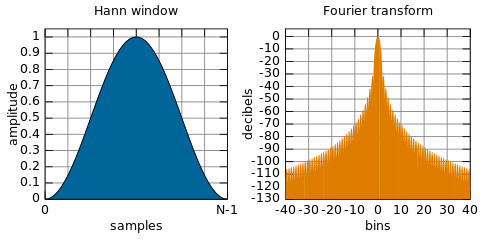
\includegraphics[width=100mm]{hann.jpg}
	\caption[Hann Window Function]{The Hann window function, and its resulting Fourier transform~\cite{Niemitalo2013}.} 
	\label{fig:hann} 
\end{figure}

\indent Having controlled for the most significant sources of potential error in the time domain, the next step is to pass the modified signal through the Fourier transform algorithm in order to obtain our frequency spectrum. But what exactly is the Fourier transform?


% --- Section 3.3 - The Fourier Transform ---
\section{The Fourier Transform}
\indent At a basic level, Fourier analysis is a branch of mathematics that deals with splitting signals into sine waves~\cite[ch. 8]{Smith1998}. The Fourier transform is a particular technique under the banner of Fourier analysis which decomposes a given signal into its constituent frequencies, providing the frequency domain representation of that signal~\cite[ch.8.1]{Smith1998}. It's an important point to take note of that this frequency domain representation actually contains exactly the same information as is contained in the original time domain representation, it is simply shown in a different form; hence the term ``transform''. There are two main features defining a signal's type: a signal can either be ``continuous'' or ``discrete'', and it can either be ``periodic'' or ``aperiodic'', and the four possible combinations of these features yields four primary categories of Fourier transform. The first type is continuous-periodic and is commonly referred to as the {\bf Fourier series}, the second is continuous-aperiodic and is usually called simply the {\bf Fourier transform}, the third is discrete-periodic and is typically called the {\bf discrete Fourier transform}, and the final one is the discrete-aperiodic {\bf discrete time Fourier transform}. The names are a bit poorly chosen and difficult to differentiate, but the important one for our purposes is the discrete Fourier transform (DFT), so let's delve a little bit deeper into that.

\indent The first thing that needs to be understood is that, since Fourier analysis deals in sinusoids (sine waves) which by definition are infinite, the four classes of signal previously mentioned all must necessarily extend to infinity in both directions; there is no version of the Fourier transform that deals in finite-length signals~\cite[ch.8.1]{Smith1998}. But in real-world audio analysis, we deal almost exclusively in non-repeating, finite-length signals, so what can be done? The solution is to make the finite signal appear infinite, by imagining that the sample that we are looking at repeats itself, \emph{ad infinitum}, in both directions. Since these imaginary samples repeat themselves, use of this technique has the byproduct of making our signal appear not only discrete but also periodic, allowing us to use the DFT where it might not otherwise seem reasonable to do so. 

\indent Another point that needs to be mentioned is that the mathematics for this process is extremely complicated, particularly in dealing with complex numbers. This is not only rather difficult to wrap one's mind around, but also potentially extremely computationally-involved, and a poorly written DFT algorithm could substantially slow down an application. However, the existence of a so-called ``fast Fourier transform'' (FFT) mitigates a number of these concerns, and one extremely powerful implementation is the library called the ``Fastest Fourier Transform in the West'' (FFTW)\footnote{\url{http://fftw.org/}}, which has been developed explicitly for the purpose of quickly, efficiently, and effectively applying Fourier transforms. This package allows us to gloss over the bulk of the mathematics and optimization details, and instead focus on the practical aspects of the FFT. 

\indent The FFTW package provides a number of modes of usage allowing a variety of input-to-output conventions, such as complex-to-complex, complex-to-real, and real-to-complex; since the data that we are capturing is purely real-valued, the real-to-complex routine applies~\cite{Frigo2005}. We begin with an input signal consisting of a series of real-valued data points in the time domain, say $N$ such points (for reasons of both convention and efficiency, $N$ is typically a power of two ranging between 32 and 4096~\cite[ch. 8.1]{Smith1998}). The resulting output once this input signal has been passed through the DFT then takes the form of an $(\frac{N}{2} + 1)$-sized array of complex numbers, with the real portion representing the amplitude of the signal's constituent cosine waves, and the imaginary portion similarly representing the signal's constituent sine wave amplitudes. From this point, for our purposes it is sufficient to know that each of the complex numbers in the output represents a frequency ``bin'', each of which covers a range of frequencies whose resolution is dependent on the input parameters, namely the sample rate $F_s$ and the DFT size $N$. For instance, using a sample rate of $F_s = 8000$ and a DFT size of $N = 4096$, each bin of the frequency spectrum will be $\frac{F_s}{N} = \frac{8000}{4096} \approx 1.95$Hz wide. If we then take a look at the magnitudes of the components of these ``bins'' (defined as the square-root of the real and imaginary portions, each squared: $\sqrt{real^2 + imaginary^2}$), we can obtain the magnitude of this frequency component.

\indent So, now that we have this frequency information, we can simply look at the bin that has the highest magnitude and our fundamental frequency will be in this $\sim2$Hz range, right? Well, not quite. While this technique, sometimes called the {\bf FFT magnitude peak} method~\cite{Nicholson2011} \emph{could} work, there are many things which could cause a particular frequency that is not the fundamental to ``spike'' -- things like harmonics, or even simply background noise -- making such a straight-forward technique quite unreliable. A more robust estimation technique needs to be used.


% --- Section 3.4 - Pitch Estimation ---
\section{Pitch Estimation}
\indent While pitch is closely related to frequency, they are not equivalent, and because of this frequency is sometimes not enough to distinguish notes. In spite of this, however, many times a frequency alone can serve to provide a reasonable enough estimate for pitch, especially for relatively simple applications such as this. But there remains the problematic fact that, to this point, we are given a wide-ranging frequency spectrum, rather than a single firm frequency value, and pin-pointing the fundamental can be an involved process. Indeed, moving from the frequency spectrum to even the ``approximate'' pitch is not a straight-forward matter of looking at the frequency-amplitude graph, comparing it against a table of frequency values for notes and octaves, and connecting them somehow\footnote{Although, such tables do certainly exist, and are essential for making the final leap to the note once we've acquired a pitch-frequency estimate. See the table at \url{http://www.seventhstring.com/resources/notefrequencies.html}, for reference.}. So what's the best way to go about getting a reasonably accurate estimation of pitch-frequency?

\indent Dozens of methods have been proposed for estimating pitch, with a wide range of results dependent on a number of factors. There are methods which use only the time-domain data, methods using only the frequency-domain data, and methods which combine the two; there are methods better suited to measuring sounds generated by human vocal chords, and some better suited to interpreting electronic sounds; some better suited to higher-frequency sounds, and some better for lower frequencies; etc.~\cite{delaCuadra-nd,Nicholson2011}. Since our task is a relatively simple one, any number of the possible methods likely would suffice -- and, indeed, a fairly large number were briefly considered -- but in the interest of limiting scope the focus was narrowed to three potential methods widely recommended by the digital audio processing community at-large\footnote{This so-called ``community at-large'' consisted of a variety of readily available sources, not terribly scientifically chosen, ranging from apparently knowledgeable and well-spoken forum users on programming and audio analysis websites, to university professors, and master's and PhD students that have written papers, or slide packs, or blog posts on the subject.} for their mix of simplicity and effectiveness: ``auto-correlation'', ``cepstrum'', and ``harmonic product spectrum''.

\subsection*{Auto-Correlation}
\indent {\bf Auto-correlation} is a process that takes advantage of the fact that the signals that we are dealing with are at least somewhat periodic in nature, and thus the signal will be very likely to have repeated behaviour after some fundamental period length~\cite{Middleton2003}. By taking some window of the audio signal that is at least large enough to capture this repetition, ``shifting'' it by some degree, and then comparing this shifted version with the original, we can calculate the so-called {\bf auto-correlation function} (ACF). By then differentiating the ACF and studying the result, the fundamental frequency can be estimated. This method as it is laid out above is performed entirely in the time domain, and so has the benefit of not requiring the calculation of the fast Fourier transform, but even without that particular computation the algorithm is still extremely expensive~\cite{delaCuadra-nd}, making use of a large number of comparisons and some fairly computationally-intensive calculus. Additionally, although this method is fairly robust in the presence of noise, it is very sensitive to sample rate~\cite{Middleton2003} and quite prone to octave errors \cite{Knesebeck2010}. There is a method for more efficiently calculating the auto-correlation by using the inverse FFT (essentially the fast Fourier transform procedure performed in reverse)~\cite{Middleton2003}, but because of its other issues, this method was discarded.
\clearpage
\subsection*{Cepstrum}
\indent The second pitch estimation technique to be examined was a process called {\bf cepstrum}, which you'll notice is just the word ``spectrum'' with its first four letters inverted. This peculiar name derives from the fact that the technique which it describes begins with the regular frequency spectrum, and then twists it about by first calculating the logarithm of the spectrum, and then applying the inverse FFT \cite{Norton2003}, as below (where $\mathcal{F}$ represents the FFT function, and $f(t)$ represents the original time-domain audio signal): 
$$| \mathcal{F}^{-1} (\; log(\;|\mathcal{F}(\;f(t)\;)|^2\;)\;)|^2$$

\indent While applying the inverse FFT to the normal spectrum would effectively just undo the original FFT application, applying it to the \emph{logarithm} of the spectrum has the effect of revealing information about the rate of change among the constituent frequencies. This technique has been demonstrated to be very effective at handling overtones and harmonics, sometimes even revealing fundamental frequencies that are not only comparatively weak, but completely obscured by harmonics, and as a result it is widely used for applications involving human speech~\cite{delaCuadra-nd}. However, cepstrum is not meant for accurate frequency estimation, and this fact coupled with the somewhat-high computational overhead inherent in performing what amounts to two Fourier transforms means that this method may not be ideal for an instrument tuner with real-time calculation concerns.

\subsection*{Harmonic Product Spectrum}
\indent Which brings us to the third pitch estimation technique that was studied, and the one which was ultimately selected: the {\bf harmonic product spectrum} (HPS). The fundamental theory behind the use of HPS for determining musical notes is that the spectrum for a given note consists of a series of peaks, each of which is either the fundamental frequency, or a harmonic frequency (i.e. some integer multiple of the fundamental). So, if the audio signal is processed in order to obtain its spectrum, and this spectrum is then compressed (or ``downsampled'') a number of times and compared against its original uncompressed self, the ``strongest'' harmonic peaks should align~\cite{Middleton2003}, revealing a common factor. Thus, if we multiply these compressed versions of the signal together the ``strongest'' harmonic peak should become amplified, and since this value will necessarily be the greatest common divisor of these signals, it stands to reason that this would be the fundamental frequency. Fig.\ref{fig:hps} below~\cite{delaCuadra-nd} provides a very good illustration of this process:
\clearpage
\begin{figure}[h]
	\centering
	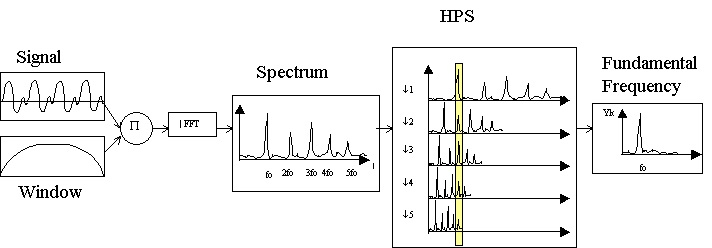
\includegraphics[width=150mm]{hps.jpg}
	\caption[HPS Diagram]{A diagram illustrating the harmonic product spectrum (HPS) process. \\\emph{(Notice the peak-alignment among the downsampled signals, and the resulting sharp spike indicating the fundamental frequency once they are multiplied together.)}} 
	\label{fig:hps} 
\end{figure}

The HPS technique has the benefit of being computationally quite inexpensive, utilizing just one instance of the fast Fourier transform and some basic multiplication. It is also reasonably resistant to ``additive and multiplicative noise''~\cite{Middleton2003}, and flexible in terms of the types of input. The primary downside, on the other hand, is that it is only as accurate as the window size that is used to calculate the FFT~\cite{Middleton2003}, and so it is necessary to balance the desire for higher frequency resolution (and thus a larger window size) against the computational savings gained over other comparable methods. Since the requirements for this particular application are not overly stringent, the balance of accuracy and speed that this method affords -- and its inherent flexibility to allow us to adjust these factors as needed -- caused the HPS technique to come out ahead of the alternatives.

\clearpage

% ___ Chapter 4 - Implementation and Configuration ___
\chapter[Implementation and Configuration]{Implementation and Configuration}
% --- Section 4.1 - Platform Information ---
\section{Platform Information}
\indent We turn now to the implementation and configuration details for the RT-Tuner program. This application was developed in Windows 8.1 as a simple Windows desktop program, and was written in the C++ programming language using the ``Visual Studio Express 2013 for Windows Desktop''\footnote{\url{https://www.visualstudio.com/en-us/products/visual-studio-express-vs.aspx}} integrated development environment (Visual Studio IDE, or just Visual Studio). As it was developed in the context of Visual Studio, the code is encapsulated in terms of a Visual Studio solution file, and loading the code should be a simple matter of opening the solution file (\emph{rt-tuner.sln}) inside of the Visual Studio IDE. The following portion of this chapter will be dedicated to discussing the steps required to properly compile and run the code, including information about the external packages which were used -- some of which require particular installation or setup, and some of which have simply had their code included into the Visual Studio solution -- and  a few words on typical IDE configuration options. The subsequent section will be devoted to understanding the general flow of the program itself, as well as information on particular configuration details for customization purposes. And finally, the last portion of this chapter will include a brief overview of how one might most easily extend this program to add or change functionality (discussion on precisely what sorts of changes might be made, however, are largely left for later chapters).
\clearpage


% --- Section 4.2 - Compiling the Code ---
\section{Compiling the Code}
% - Subsection 4.2.1 - External Packages -
\subsection*{External Packages}
\indent As suggested above, the first couple external packages require some effort to install and/or configure, and it is hoped that by including the following information this process will be made as smooth as possible. First is the GUI package called {\bf wxWidgets}\footnote{\url{https://www.wxwidgets.org/}}. The following step-by-step instructions explain the simplest method that was found to install this package:

\indent({\footnotesize\bf Note: It's important to note that both the download size, and uncompressed installation size of this library are quite substantial, so it is strongly recommended to have access to a fast internet connection and at least 5GB of free hard disk space available before proceeding.)}

\begin{enumerate}
	\item Download the package called {\bf wxPack} from the GitHub repository located at \url{https://github.com/rjpcomputing/wxpack/wiki}. This can be done by following the download link in the ``News'' posting dated 07/22/2014 for the wxPack release supporting wxWidgets v3.0.1, and obtaining the \\
	{\bf wxPack\_v3.0.01.00.exe} file. \\(As noted above, this package is very large ($\sim1$~GB), and so it can take some time to download.)
	\item Run the executable to install the package somewhere on your hard disk (e.g. ``c:\textbackslash wxWidgets3.0\textbackslash''), making sure to install the ``Microsoft Visual C++ 2013'' items, at minimum. 
	\item Once this is completed, it will be necessary to set a Windows environment variable to ensure that Visual Studio can properly refer to the items included in this package. This can most easily be done by doing the following:
	\begin{enumerate}
		\item Open the Windows {\bf Control Panel}, browse to the {\bf System and Security} section, and open the {\bf System} page.
		\item From here, click on the {\bf Advanced System Settings} link on the left-hand side, go to the {\bf Advanced} tab, click on the {\bf Environment Variables} button.
		\item Under the {\bf Environment variables for {\em \textless username\textgreater}} section (where {\em \textless username\textgreater} is your username), click the {\bf New...} button.
		\item Enter ``WXWIN'' (without quotation marks) for the variable name, and the installation path you used above (i.e. ``c:\textbackslash wxWidgets3.0\textbackslash'') for the variable value, and click {\bf OK}. You can ensure that this was done correctly by verifying that the environment variable is now listed in the {\bf Environment variables for {\em \textless username\textgreater}} box.
	\end{enumerate}
\end{enumerate}

\indent That's it, the wxWidgets package should now be installed properly. The next package which might require some degree of setup is the {\bf Fastest Fourier Transform in the West}\footnote{\url{http://www.fftw.org/download.html}} (FFTW). An import library (\emph{libfftw3-3.lib}) is included with the source code, but depending on your platform and development environment, it may be necessary to generate a new one in order to properly link to the dynamic link library (DLL) files for this package in Visual Studio. This can be done by running the ``lib'' command that is included in Visual Studio targeting the \emph{.def} file included in the FFTW package (e.g. ``\textless path\textgreater\textbackslash rt-tuner\textbackslash phase1\textbackslash fftw\textbackslash libfftw3-3.def'', where ``\textless path\textgreater'' is the installation path for the rt-tuner project). This process is explained in the FFTW documentation~\cite{Frigo-nd}, but I've provided the necessary steps for this portion below, for easy reference:

\begin{enumerate}
	\item Open a windows command prompt (this can be done in several ways, most simply by clicking {\bf Start} $\rightarrow$ {\bf Run...}, typing \emph{cmd} and then clicking {\bf OK}).
	\item Browse to the Visual C ``bin'' directory of the Visual Studio installation, e.g.:
		\begin{itemize} \item \emph{\textgreater cd c:\textbackslash Program Files\textbackslash Microsoft Visual Studio 12.0\textbackslash VC\textbackslash bin\textbackslash} \end{itemize}
	\item Run the ``lib'' command, targeting the correct \emph{.def} file, e.g.:
		\begin{itemize} \item \emph{\textgreater lib /def:``\textless path\textgreater\textbackslash rt-tuner\textbackslash phase1\textbackslash fftw\textbackslash libfftw3-3.def''} \end{itemize}
	\item Move the ``libfftw3-3.lib'' and ``libfftw3-3.exp'' files that are created into the FFTW folder in the project directory, e.g.: 
		\begin{itemize}
			\item \emph{\textgreater move libfftw3-3.lib ``\textless path\textgreater\textbackslash rt-tuner\textbackslash phase1\textbackslash fftw\textbackslash''}
			\item \emph{\textgreater move libfftw3-3.exp ``\textless path\textgreater\textbackslash rt-tuner\textbackslash phase1\textbackslash fftw\textbackslash''}
		\end{itemize}
\end{enumerate}

\indent (It should be noted that moving the \emph{.lib} and \emph{.exp} files is not strictly necessary, as we could tell Visual Studio to look for the library wherever we like, but relative paths have been used in the Visual Studio solution file for this project, and so this is where it will look for this library by default.) Now, with the wxWidgets package and the FFTW library set up, the most difficult part is behind us.

\indent The remaining external packages which were used require no particular action to facilitate compilation, and are simply included as additional code in the solution itself. The first such package is the {\bf RtAudio} audio input/output package\footnote{\url{http://www.music.mcgill.ca/~gary/rtaudio/}}, which includes the \emph{audioprobe.cpp} file and all files under the \emph{RtAudio} sub-directory. This package's purpose is to interface with the microphone, and handle the capturing of the live audio. The next two packages, {\bf wxMathPlot}\footnote{\url{http://wxmathplot.sourceforge.net/index.shtml}} and {\bf kwxIndustrialControls}\footnote{\url{http://wxcode.sourceforge.net/showcomp.php?name=kwxIndustrialIndicators}}, include the files located under the \emph{wxmathplot} and \emph{kwic} sub-directories, respectively. These packages are extensions to the wxWidgets GUI package, with the wxMathPlot package being used to draw and control the spectrum graph, and the kwxIndustrialControls package used to draw and control the tuner's needle gauge.

% - Subsection 4.2.2 - IDE Configuration -
\subsection*{IDE Configuration}
\label{sec:ideconfig}
\indent With all of the external packages installed and configured, the IDE must now be told which items to use and where to find them, as well as being told any other relevant details about this project. Due to the fact that this project was configured in such a way that it uses environment variables and local paths, these particulars should ideally already be taken care of for you by simply opening the aforementioned \emph{rt-tuner.sln} file in Visual Studio. However, in the event that something has gone wrong, or some tweaks need to be made, the full file include list and IDE configuration profile is laid out in Appendix \ref{app:ide}. Unfortunately, since the only development environment that was used throughout the development of this project was the aforementioned Visual Studio build (more specifically, Microsoft Visual Studio Express 2013 for Windows Desktop, Version 12.0.31101.00 Update 4), no guarantees can be made with respect to compiling the code under any other environment.


% --- Section 4.3 - Code Structure and Configuration Details ---
\section{Code Structure and Configuration Details}
\indent Looking at the code structure itself, the RT-Tuner project is divided into 4 discrete parts: the {\bf RTTuner} driver, the {\bf AudioVisualizer}, the {\bf AudioCapturer}, and the {\bf AudioProcessor}. The \emph{RTTuner.cpp} driver class's purpose is simply to kick off the entire program by initializing the AudioVisualizer. The \emph{AudioVisualizer.cpp} class is responsible for a significant portion of the functionality, handling all of the graphical elements, as well as launching and controlling the AudioCapturer, and converting the data received from the Capturer into a display-friendly format. The \emph{AudioCapturer.cpp} class's responsibility is to interface with the host computer's audio devices, capturing an audio signal, sending this audio data through the AudioProcessor, and then returning the results to the Visualizer. Finally, we have the \emph{AudioProcessor.cpp} class which is responsible for the majority of the calculations which are performed on the captured audio data, including applying the windowing and filter functions and calculating the FFT. Each class acts relatively independently, using fairly simple API functions to communicate with each other and pass data back and forth.

\indent As mentioned, the RTTuner driver class is fairly straight-forward, consisting of only a few lines of code and largely serving only to kick-off the AudioVisualizer. The Visualizer, however, is rather more complicated. Upon initialization, the Visualizer sets up all of the necessary GUI elements for the program, such as creating a tabbed interface with a graph for the frequency spectrum on one tab (``Spectrum''), and a needle gauge and text display label for the tuner on the other tab (``Tuner''), and also creating a button at the bottom of the window for controlling the audio capture stream (see Fig.~\ref{fig:gui}). The Visualizer also configures and launches an instance of the AudioCapturer in its initialization, passing it parameters for keeping track of the frequency estimations. Once up and running, the Visualizer uses a timer to periodically refresh the relevant GUI elements (i.e. the spectrum graph, needle gauge, and tuner label), including using a method to calculate the musical note corresponding to the most recently estimated average fundamental frequency.

\begin{figure}[h]
	\centering
	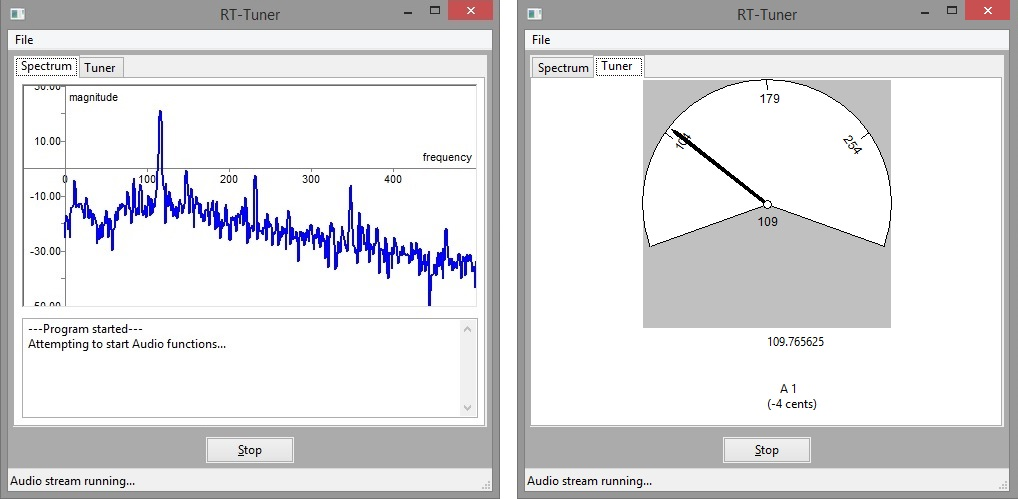
\includegraphics[width=140mm]{visualizer.jpg} \\
	\caption[RT-Tuner GUI]{The graphical user interface generated by the AudioVisualizer class.} 
	\label{fig:gui} 
\end{figure}	

\indent The next most complicated class is the AudioCapturer, which makes heavy use of the RtAudio audio input/output API. Upon initialization, the AudioCapturer instantiates an AudioProcessor, and then uses some pre-determined constant values -- like the number of audio channels to consider, the audio sample rate to use, and the number of frames to capture at a time -- to configure the computer's default audio input device and open a capturing stream. The Capturer contains a few functions to start, stop, or close the audio stream, but once the stream is running the bulk of the action takes place in the {\bf CaptureAudio()} audio callback function. The CaptureAudio() function is a function which is called every time the audio stream has captured the pre-determined number of frames, and it is inside this function that the AudioProcessor is used in order to examine and manipulate the raw audio data to acquire the results that we are looking for. In this case, the raw audio data first has a low-pass filter applied to it (twice, for good measure), then a Hanning window, and then the FFT is performed in order to obtain the frequency spectrum data, which is then passed back to the Visualizer in the form of a vector to be displayed on the ``Spectrum'' graph. At this point, the spectrum data is also used by the AudioProcessor's harmonic product spectrum algorithm in order to calculate the likely fundamental frequency, which is then passed back to the Visualizer in such a way that we can accumulate the fundamental frequency data and average the results over time. It's important to note that the callback function is necessarily a static method, and so a special structure is required to provide it access to important information; in particular, an instance of a \emph{struct} object is passed to the callback, containing references to the AudioProcessor instance, the AudioVisualizer's graph vector, and a pair of variables for the frequency accumulation.

\indent The final component of the project to be considered is the calculation-heavy AudioProcessor class. This class is fairly lightweight in terms of code, consisting of only five short methods, but this is where the most sophisticated algorithms reside. In the context of this application, the first methods that are used are for the low-pass filter, with one method using some input values to pre-calculate the parameters which are to be used for the filter, and the second method actually applying this filter. (Note that the algorithms used for these two methods were written by Bjorn Roche\footnote{The code for these was found by following the link in his blog post here: \url{http://blog.bjornroche.com/2012/07/frequency-detection-using-fft-aka-pitch.html}}, and are borrowed and used here with absolutely no claim of credit.) The next method is very short, only about three lines of code, consisting only of a loop which performs the Hanning window calculation\footnote{\url{https://en.wikipedia.org/wiki/Hann_function}} on each data point in the supplied input array. The next method to be used is perhaps the most complicated of these (at least in terms of its effect, if not necessarily its implementation), using the previously-mentioned FFTW package to determine an efficient real-to-complex calculation plan and perform the fast Fourier transform, then taking the resulting complex-number output data and calculating and returning the magnitude of this spectrum data. The final method included in this class is the HPS algorithm, which takes as input an array of spectrum data and a downsampling factor, performs the specified number of downsampling operations, and multiplies the resulting compressed spectra together. The result is then searched for a peak, this peak is double-checked in an attempt to minimize the likelihood of harmonics yielding a false positive for the fundamental frequency~\cite{delaCuadra2001}, and the bin number in which the true frequency peak was found is then returned, allowing the calling function to pinpoint the likely fundamental frequency.

\indent Looking a bit more deeply into the code, there are a few particular configuration options that are of interest depending on the context in which the program will be used. A list of relevant configuration variables is provided below, containing indications of where to find the variable, a brief description of its purpose, its default value, and, where appropriate, a short discussion of the rationale for the default and alternative values.

\begin{itemize}
	\item File: \emph{AudioVisualizer.h}
	\begin{itemize}
		\item {\bf REFRESH{\_}INTERVAL} (default: 100) -- \emph{The length of time, in milliseconds, between GUI refreshes.}
	\end{itemize}
\clearpage
	\item File: \emph{AudioCapturer.h}
	\begin{itemize}
		\item {\bf AUDIO{\_}NUM{\_}CHANNELS} (default: 1) -- \emph{The number of audio channels to capture. (Currently untested with more than 1 channel.)}
		\item {\bf AUDIO{\_}SAMPLE{\_}RATE} (default: 8000) -- \emph{The number of audio samples to capture per second.}\\
		$\rightarrow$ The higher this number is the more detail is captured, but there is a performance trade-off. A sample rate of 44100 Hz is roughly equivalent to the quality of an audio CD, and 8000 Hz is approximately equivalent to a telephone or walkie-talkie. Since a tuner is only concerned with fundamental frequencies which tend to be on the low-end of the spectrum, it is typically quite safe to sacrifice sound quality in favour of computational efficiency.
		\item {\bf AUDIO{\_}BUFFER{\_}FRAMES} (default: 4096) -- \emph{The number of frames to capture at a time before calling the RtAudio callback function.}\\
		$\rightarrow$ Each frame consists of AUDIO{\_}SAMPLE{\_}RATE samples. A smaller value will reduce the time delay between processing packets of data but will also yield much lower frequency resolution (and \emph{vice versa} when using a larger value). In order to assure maximum efficiency for the FFT algorithm (among other things), this value should ideally be a power of two.
		\item {\bf AUDIO{\_}DOWNSAMPLE{\_}FACTOR} (default: 4) -- \emph{The number of downsampling iterations to perform for the HPS algorithm.}
		\item {\bf MAX{\_}FREQ} (default: 330) -- \emph{The maximum frequency to consider.}
		\item {\bf MIN{\_}FREQ} (default: 29) -- \emph{The minimum frequency to consider.}\\
		$\rightarrow$ The MIN{\_}FREQ/MAX{\_}FREQ parameters are used for two primary purposes: to set the bounds of the needle gauge scale, and to set the passband for the low-pass filter.
	\end{itemize}
\end{itemize}


% --- Section 4.4 - Extending RT-Tuner ---
\section{Extending RT-Tuner}
\indent Keeping in mind the background that has been discussed thus far regarding the configuration and structure of the RT-Tuner application, there appear to be two primary areas where the program could be extended. The first such area is in the AudioProcessor, where any number of methods could be added in order to perform a variety of manipulations of the raw audio data, and the second is in the AudioVisualizer, where graphical interface elements could be added or changed for a variety of purposes.

\indent Making such changes to the AudioProcessor would be a simple matter of adding the aforementioned methods to the \emph{AudioProcessor.h} and \emph{AudioProcessor.cpp} files, and then adding the code to call them in the ``CaptureAudio()'' callback function located in the \emph{AudioCapturer.cpp} class. Ideally, the data generated by these new methods would be compatible with the existing GUI elements, which would mean that it would simply be a matter of using the existing graph vector and frequency variables to pass this information back to the Visualizer for display---however if this is not the case then some more significant customization will be necessary. In such a case, the {\bf userdata} structure located in the \emph{AudioCapturer.h} header file could prove useful in relaying the information back to the AudioVisualizer, by virtue of adding additional reference variables to the structure and updating the constructors for the structure itself as well as the AudioCapturer class. Of course, the AudioVisualizer will also need to be updated to be able to retrieve this information, perhaps by adding instance variables to the \emph{AudioVisualizer.h} header file similar to the existing ``dataLayer'' vector or ``totalFreq'' variable, and passing references to these to the AudioCapturer initialization (which is done at the end of the AudioVisualizer constructor).

\indent If additional GUI widgets are desired -- whether for the display of new data generated through the process just described, or simply in the interest of improving the existing interface -- adding them should be a fairly simple matter, especially given the very useful wxWidgets documentation\footnote{\url{https://www.wxwidgets.org/docs/}}. For any given GUI widget, there are likely to be three main areas of concern: definition/initialization, refreshing, and event handling. The definition and initialization portion is a fairly straight-forward matter of adding relevant variables to the \emph{AudioVisualizer.h} header file, and then configuring and placing the elements in the AudioVisualizer's constructor in the \emph{AudioVisualizer.cpp} file\footnote{Note that details regarding particular wxWidgets elements and window organization is beyond the scope of this document, but there are many useful tutorials to be found in the wxWidgets documentation and elsewhere online.}. Refreshing concerns are similarly simple, as one needs only to add code to the ``RefreshWindow()'' method of the \emph{AudioVisualizer.cpp} class to make whatever updates are required upon window refresh. Events, however, are rather more complicated. Many widgets won't require dedicated event handlers, but in the event that one is required the following steps should be followed:

\begin{enumerate}
	\item Add an entry for this event to the enumeration of unique identifiers at the top of the \emph{AudioVisualizer.cpp} file, e.g.:
\begin{lstlisting}[language=C++,title=\emph{AudioVisualizer.cpp}]
enum {
	ID_QUIT = wxID_HIGHEST,
	[...]
	ID_REFRESH_TIMER,
	ID_MYEVENT
};
\end{lstlisting}
\clearpage
	\item Add a prototype for an event handler method to the \emph{AudioVisualizer.h} header file, and write the corresponding method in the \emph{AudioVisualizer.cpp} class file, e.g.:
\begin{lstlisting}[language=C++,title=\emph{AudioVisualizer.h}]
class AudioVisualizer : public wxFrame 
{
public:
[...]
	// -- event handlers
	[...]
	void	OnRefreshTimer(wxTimerEvent& event);
	void	OnMyEvent(wxCommandEvent& event);
	[...]
}
\end{lstlisting}
\begin{lstlisting}[language=C++,title=\emph{AudioVisualizer.cpp}]
void AudioVisualizer::OnMyEvent(wxCommandEvent& event)
{
	// code for handling the event goes here
}
\end{lstlisting}
	\item Map the unique identifier from step 1 to the event handler method created in step 2 in the wxWidgets ``Event Table'' at the top of the \emph{AudioVisualizer.cpp} file.\\
	$\rightarrow$ Note that a particular type of event will need to be specified here (e.g. EVT{\_}BUTTON, EVT{\_}TIMER, etc.). A list of viable options can be found in the wxWidgets documentation\footnote{\url{http://docs.wxwidgets.org/trunk/group__group__funcmacro__events.html}}.
\begin{lstlisting}[language=C++,title=\emph{AudioVisualizer.cpp}]
// -- event table
BEGIN_EVENT_TABLE(AudioVisualizer, wxFrame)
  [...]
  EVT_ANY(ID_MYEVENT, AudioVisualizer::OnMyEvent)
END_EVENT_TABLE()
\end{lstlisting}
\end{enumerate}
\clearpage

\indent Although there may be additional tweaks and adjustments required depending on exactly what the goal is, the above should provide a decent start. In general, there are only a handful of sections of the code that may need to be modified in order to provide these types of additional functionality:
\begin{itemize}
	\item \emph{AudioProcessor.h} header:\\	
		-- To define new audio evaluation and manipulation methods.
	\item \emph{AudioProcessor.cpp} class:\\	
		-- To implement new audio evaluation and manipulation methods.
	\item \emph{AudioCapturer.h} header:\\
		$\rightarrow$ {\bf userdata} structure -- To accommodate passing new information to the AudioVisualizer.
	\item \emph{AudioCapturer.cpp} class:\\
		$\rightarrow$ {\bf CaptureAudio()} callback -- To call additional AudioProcessor methods, and/or pass information to the AudioVisualizer.\\
		$\rightarrow$ {\bf AudioCapturer()} constructor -- To accommodate passing new information to the AudioVisualizer.
	\item \emph{AudioVisualizer.h} header:\\ 
		-- To accommodate receiving new information from the AudioCapturer.\\
		-- To define new GUI elements.\\
		-- To define event handler methods.
	\item \emph{AudioVisualizer.cpp} class:\\
		-- To uniquely identify event handlers, implement event handler methods, and map event handler methods to their unique identifier.\\
		$\rightarrow$ {\bf AudioVisualizer()} constructor -- To accommodate receiving new information from the AudioCapturer, and/or add new GUI elements.\\
		$\rightarrow$ {\bf RefreshWindow()} method -- To update/refresh GUI display information.
\end{itemize}
\clearpage


% ___ Chapter 5 - Results ___
\chapter{Results}
\indent As intended, this project yielded a passable audio analysis tool, which could be used to at least crudely aid in the tuning of an instrument. Having tested the end product with a tone generator using frequencies ranging from about $30$--$330$Hz, the spectrum display appeared to show a reasonable spread of frequency data given the input tones, however gauging the accuracy of the spectrum through inspection is a very difficult thing to accomplish, and so no reliable judgment can be made of this. Far more encouraging are the results with respect to the needle gauge and note information display: the program often only took a matter of seconds to ``lock on'' to a fundamental frequency, and once stabilized in this manner the program consistently displayed a fundamental frequency estimation that was within approximately 2Hz of the true value indicated by the tone generator. Also, the note conversion calculation, and cent offset appeared to be well within acceptable degrees of error for this program's purpose. This is especially encouraging given that it was the case even despite the use of a poor quality laptop microphone and occasional background noise. However, the results were not all good: the successes described above were only witnessed when using frequencies in the range of about $100$--$330$Hz; any frequency higher or lower than this range would cause the program to fail to lock on to any particular value, with the tuner needle and note estimation constantly jumping around (although anything higher than $330$Hz \emph{should} fail, due to the low-pass filter). 

\indent With respect to the design decisions which were made along the way, there are similarly mixed results. From a GUI perspective, the two-dimensional spectrum graph proved to be less useful than expected, as the frequently-changing frequency landscape rarely yielded much in terms of useful information in the graph. Even in the few instances where clear, steady peaks were witnessed, the presence of harmonics and noise, etc., rendered the information less than useful. Similarly, the tuner's needle gauge as implemented is less useful than it should be. As mentioned in Chapter \ref{sec:vissnd} above, the ideal scenario would have the gauge re-calibrate its scale dependent on the nearest detected note, but the decision to confine the gauge to one large, static frequency range limited the precision and proved more useful in determining frequency at a glance, rather than the intended goal of effectively getting across the pitch/note information. Regarding the note information, however, the text label approach seemed to work very well. One other thing that seemed to work very well, given the successes mentioned in the previous paragraph, was the decision to use the harmonic product spectrum algorithm to estimate pitch. The program appeared to yield quite accurate results, and to do so quite quickly with no noticeable impact on the CPU usage of the test-bed computer.

\indent Ultimately, this application met its stated goals, but there are many ways in which things could be improved upon, and many alternative directions that could be taken in the future. Some potential areas of improvement include: use of a better recording mechanism, for instance a higher-quality microphone; improved encapsulation and reduced cohesion, to make the program safer and more extensible; support for expanded frequency ranges; and fixing procedural mistakes, for instance the calculation of the parameters for the low-pass filter is currently performed repeatedly, when it really only needs to be done once. With respect to possible future expansions on this subject, it would be a fairly simple matter to add functionality for a number of other windowing, filtering, and pitch detection techniques, allowing for a comparison of their effectiveness. Or, broadening the scope slightly, the pitch detection capabilities could be applied to performing sound transformation, e.g. pitch-shifting, time-scaling, etc., or perhaps some sort of music notation program, recording live music as sheet music, for example. 
\clearpage

% ___ Chapter 6 - Conclusion ___
\chapter{Conclusion}
\indent In the end, the RT-Tuner program has accomplished what it was supposed to: it is a reasonably effective real-time audio analysis tool with a user-friendly interface, and the capability of fairly accurately estimating musical pitch. It has its share of flaws, ranging from GUI design failings to frequency range restrictions to coding mistakes, but such things are relatively easily fixed, and the speed and accuracy of the results obtained even in spite of these flaws is more than enough to meet the threshold for success -- not to mention being very encouraging with regard to future potential. It is hoped that the design of this application, and the foundational skeleton that has been developed here, is sufficiently robust and flexible as to be easily built upon. Audio analysis remains a complex, dynamic, ever-expanding domain of study, and while this tiny contribution is nothing new or profound, perhaps it could prove useful in building something that is.
\clearpage

%%%%%%%%%%%%%%%%%%%%%%%%%%%%%%%%%%%%%%%%%%%
%	BACK MATTER
%%%%%%%%%%%%%%%%%%%%%%%%%%%%%%%%%%%%%%%%%%%

%------------------------------------------
%	REFERENCES
%------------------------------------------
% Switch to the Reference headers
\referenceheaders
\begin{thebibliography}{100}
	% References:
	\bibitem[Anon,~2014a]{Anon2014a} Anon (2014, November 8). ``Tech Stuff - Frequency Ranges''. \emph{ZyTrax Communications Home Page}. Retrieved March 29, 2015 from \url{http://www.zytrax.com/tech/audio/audio.html}

	\bibitem[Anon,~2014b]{Anon2014b} Anon (2014, July 8). [Waveform and spectrum of the union of two sine waves]. ``Time and Frequency Domain''. \emph{Erzetich - Handcrafted Headphone Amplifiers}. Retrieved on April 3, 2015 from \url{http://www.erzetich-audio.com/knowledgebase-05-time-vs-frequency}

	\bibitem[Anon,~2014c]{Anon2014c} Anon (2014, July 8). [Waveform and spectrum of an uncertain configuration of frequencies]. ``Time and Frequency Domain''. \emph{Erzetich - Handcrafted Headphone Amplifiers}. Retrieved on April 3, 2015 from \url{http://www.erzetich-audio.com/knowledgebase-05-time-vs-frequency}

	\bibitem[Audacity Wiki,~n.d.]{Audacity-nd} Audacity Wiki (n.d.). ``Sample Rates''. \emph{Audacity Wiki}. Retrieved March 18, 2015 from \url{http://wiki.audacityteam.org/wiki/Sample_Rates}

	\bibitem[Bernard and Domeier,~2001]{Bernard2001} Bernard, B., Domeier, T. (2001). ``Audio Parameters''. In \emph{Digital Media Software Development Kit Programmer's Guide} (ch.8). Retrieved March 21, 2015 from \url{http://techpubs.sgi.com/library/tpl/cgi-bin/getdoc.cgi?coll=0650&db=bks&srch=&fname=/SGI_Developer/DMSDK_PG/sgi_html/ch08.html}

	\bibitem[Bird,~1998]{Bird1998} Bird, I.W. (1998). ``Frequency to Note Calculator''. \emph{Wes Bird's Home Page}. Retrieved February 20, 2015 from \url{http://www.birdsoft.demon.co.uk/music/notecalc.htm}
	
	\bibitem[Bristow-Johnson,~n.d.]{BristowJohnson-nd} Bristow-Johnson, R. (n.d.). \emph{Cookbook formulae for audio EQ biquad filter coefficients}. Retrieved February 27, 2015 from \url{http://www.musicdsp.org/files/Audio-EQ-Cookbook.txt}
	
	\bibitem[Chisholm,~1911]{Chisholm1911} Chisholm, H., ed. (1911). ``Harmonic''. \emph{Encyclop\ae dia Britannica, 11th ed.}. Cambridge University Press. Retrieved April 5, 2015 from \url{https://en.wikisource.org/wiki/1911_Encyclop%C3%A6dia_Britannica/Harmonic}
	
	\bibitem[de~la~Cuadra,~n.d.]{delaCuadra-nd} de la Cuadra, P. (n.d.). ``Pitch Detection Methods Review'' [Paper]. Retrieved March 12, 2015 from \url{https://ccrma.stanford.edu/~pdelac/154/m154paper.htm}
	
	\bibitem[de~la~Cuadra et al.,~2001]{delaCuadra2001} de la Cuadra, P., Master, A., Sapp, C. (2001). \emph{Efficient Pitch Detection Techniques for Interactive Music}, Proceedings of ICMC 2001, International Computer Music Conference, La Habana, Cuba, September 2001. Retrieved March 17, 2015 from \url{https://ccrma.stanford.edu/~pdelac/research/MyPublishedPapers/icmc_2001-pitch_best.pdf}
	
	\bibitem[Frigo and Johnson,~n.d.]{Frigo-nd} Frigo, M., Johnson, S.G. (n.d.). \emph{FFTW}. Retrieved April 15, 2015 from \url{http://fftw.org/#documentation}
	
	\bibitem[Frigo and Johnson,~2005]{Frigo2005} Frigo, M., Johnson, S.G. (2005). \emph{The Design and Implementation of FFTW3}, Proceedings of the IEEE 93 (2), 216--231 (2005). Invited paper, Special Issue on Program Generation, Optimization, and Platform Adaptation. Retrieved April 4, 2015 from \url{http://www.fftw.org/fftw-paper-ieee.pdf}
	
	\bibitem[Hartmann,~1997]{Hartmann1997} Hartmann, W.M. (1997). \emph{Signals, Sound, and Sensation}. Springer.

	\bibitem[Hass,~2003]{Hass2003} Hass, J. (2003). ``How do we perceive pitch?''. \emph{An Acoustics Primer}, ch.12. Indiana University Website. Retrieved April 3, 2015 from \url{http://www.indiana.edu/~emusic/acoustics/pitch.htm}

	\bibitem[Middleton,~2003]{Middleton2003} Middleton, G. (2003, December 17). ``Pitch Detection Algorithms''. \emph{OpenStax CNX}. Retrieved February 10, 2015 from \url{http://cnx.org/contents/8b900091-908f-42ad-b93d-806415434b46@2/Pitch_Detection_Algorithms}

	\bibitem[Nicholson,~2011]{Nicholson2011} Nicholson, R. (2011, October 2). ``Frequency/Pitch Measurement/Estimation Techniques''. \emph{Ron's Digital Signal Processing Page}. Retrieved March 27, 2015 from \url{http://www.nicholson.com/rhn/dsp.html#1}

	\bibitem[Niemitalo,~2013]{Niemitalo2013} Niemitalo, O. (2013, February 13). ``Window function and frequency response - Hann''. \emph{Wikimedia Commons}. Retrieved March 30 from \url{https://commons.wikimedia.org/wiki/File:Window_function_and_frequency_response_-_Hann.svg}
	
	\bibitem[Norton and Karczub,~2003]{Norton2003} Norton, M.P., Karczub, D. (2003, November 17). \emph{Fundamentals of Noise and Vibration Analysis for Engineers}. Cambridge University Press.
	
	\bibitem[Park,~2009]{Park2009} Park, T.H. (2009). \emph{Introduction to Digital Signal Processing: Computer Musically Speaking}. World Scientific. Retrieved March 12, 2015 from \url{https://books.google.ca/books/about/Introduction_to_Digital_Signal_Processin.html?id=5LUuUglM5b8C}
	
	\bibitem[Qehn,~n.d.]{Qehn-nd} Qehn (n.d.). ``Calculating Frequency of Pitches''. \emph{Building the Global Orchestra: World Peace Through The Appropriation of Other Musical Cultures}. Retrieved February 17, 2015 from \url{http://members.efn.org/~qehn/global/building/cents.htm}
	
	\bibitem[Randel,~2003]{Randel2003} Randel, D.M., ed. (2003). ``Set theory''. \emph{The Harvard Dictionary of Music}. Harvard.

	\bibitem[Roche,~2012a]{Roche2012a} Roche, B. (2012, July 22). ``Frequency detection using the FFT (aka pitch tracking) With Source Code'' [Blog post]. Retrieved April 1, 2015 from \url{http://blog.bjornroche.com/2012/07/frequency-detection-using-fft-aka-pitch.html}
	
	\bibitem[Roche,~2012b]{Roche2012b} Roche, B. (2012, August 23). ``Basic Audio EQs'' [Blog post]. Retrieved April 1, 2015 from \url{http://blog.bjornroche.com/2012/08/basic-audio-eqs.html}
	
	\bibitem[Seventh~String,~n.d.]{SeventhString-nd} Seventh String (n.d.). ``Note Frequencies''. \emph{Seventh String Software}. Retrieved January 22, 2015 from \url{http://www.seventhstring.com/resources/notefrequencies.html}
	
	\bibitem[Smith,~1998]{Smith1998} Smith, S.W. (1998). \emph{The Scientist and Engineer's Guide to Digital Signal Processing}. Retrieved April 8, 2015 from \url{http://www.dspguide.com/pdfbook.htm}
	
	\bibitem[Suits,~n.d.]{Suits-nd} Suits, B.H. (n.d.). ``Making Sense of Cents''. \emph{Physics of Music - Notes}. Retrieved April 15, 2015 from \url{http://www.phy.mtu.edu/~suits/cents.html}
	
	\bibitem[von~dem~Knesebeck and Z{\"o}lzer,~2010]{Knesebeck2010} von dem Knesebeck, A., Z{\"o}lzer, U. (2010). \emph{Comparison of Pitch Trackers For Real-Time Guitar Effects}, Proceedings of the \nth{13} International Conference on Digital Audio Effects (DAFx-10), Graz, Austria , September 6--10, 2010. Retrieved March 24, 2015 from \url{http://dafx10.iem.at/proceedings/papers/VonDemKnesebeckZoelzer_DAFx10_P102.pdf}

	\bibitem[Zawistowski and Shah,~n.d.]{Zawistowski-nd}  Zawistowski, T., Shah, P. (n.d.). ``An Introduction to Sampling Theory''. Retrieved April 3, 2015 from \url{http://www2.egr.uh.edu/~glover/applets/Sampling/Sampling.html}

	\end{thebibliography}
\clearpage

%------------------------------------------
%	APPENDICES
%------------------------------------------
% Go back to using chapter headers
\chapterheaders
% Add horizontal separators to the Table of Contents, List of Figures, and List of Tables before the Appendix content:
\addtocontents{toc}{\protect\addvspace{20pt}\hrule\protect\addvspace{10pt}}
\addtocontents{lof}{\protect\addvspace{20pt}\hrule\protect\addvspace{10pt}}
\addtocontents{lot}{\protect\addvspace{20pt}\hrule\protect\addvspace{10pt}}
% Hide Appendix sections and subsections from the table of contents, displaying only chapter names
%\addtocontents{toc}{\protect\setcounter{tocdepth}{0}}

\begin{appendices}
	% Get rid of page number for the Appendix page
	\pagenumbering{gobble}
	\appendixpage
	% Use special numbering for Appendices
	\appendixpagenumbering
	\appendixfigurenumbering
	
	% ___ Appendix A - IDE Configuration Details ___
	\chapter[IDE Configuration Details - VS Express 2013]{IDE Configuration Details - \\Visual Studio Express 2013}
	\label{app:ide}
	\setcounter{figure}{0}
	\setcounter{table}{0}

	\indent As mentioned in Chapter \ref{sec:ideconfig} above, the IDE configuration details should already be taken care of in the \emph{rt-tuner.sln} solution file, but in the event of a problem, a list of the necessary file includes is provided here, along with a series of itemized lists of the notable configuration options. Importing the files should be a fairly straight-forward process ({\bf Project} $\rightarrow$ {\bf Add Existing Item...}). The IDE configuration settings can be adjusted by opening the project's properties menu ({\bf Debug} $\rightarrow$ {\bf phase1 Properties...}), changing the {\bf Configuration} to the appropriate value at the top of the \emph{phase1 Property Pages} window (``All Configurations'', ``Debug'', or ``Release''), and following along with the tree structure indicated in the upcoming sections. (\underline{Note}: Pay careful attention to the \emph{Preprocessor Definitions} items, as there are some which use multiple underscores in succession, and it is not always obvious at a glance.)

    % --- Appendix A.1 - File Include List ---
	\section{File Include List}
	Here is the full list of files which must be included in the Visual Studio solution:
	\begin{itemize}
		\item \underline{Header Files}:
		\begin{itemize}
			\item {\bf asio.h} (\emph{rt-tuner\textbackslash phase1\textbackslash rtaudio\textbackslash asio.h})
			\item {\bf asiodrivers.h} (\emph{rt-tuner\textbackslash phase1\textbackslash rtaudio\textbackslash asiodrivers.h})
			\item {\bf asiodrvr.h} (\emph{rt-tuner\textbackslash phase1\textbackslash rtaudio\textbackslash asiodrvr.h})
			\item {\bf asiosys.h} (\emph{rt-tuner\textbackslash phase1\textbackslash rtaudio\textbackslash asiosys.h})
			\item {\bf AudioCapturer.h} (\emph{rt-tuner\textbackslash phase1\textbackslash AudioCapturer.h})
			\item {\bf AudioProcessor.h} (\emph{rt-tuner\textbackslash phase1\textbackslash AudioProcessor.h})
			\item {\bf AudioVisualizer.h} (\emph{rt-tuner\textbackslash phase1\textbackslash AudioVisualizer.h})
			\item {\bf fftw3.h} (\emph{rt-tuner\textbackslash phase1\textbackslash fftw\textbackslash fftw3.h})
			\item {\bf ginclude.h} (\emph{rt-tuner\textbackslash phase1\textbackslash rtaudio\textbackslash ginclude.h})
			\item {\bf iasiodrv.h} (\emph{rt-tuner\textbackslash phase1\textbackslash rtaudio\textbackslash iasiodrv.h})
			\item {\bf iasiothiscallresolver.h} (\emph{rt-tuner\textbackslash phase1\textbackslash rtaudio\textbackslash iasiothiscallresolver.h})
			\item {\bf mathplot.h} (\emph{rt-tuner\textbackslash phase1\textbackslash wxmathplot\textbackslash mathplot.h})
			\item {\bf RtAudio.h} (\emph{rt-tuner\textbackslash phase1\textbackslash rtaudio\textbackslash RtAudio.h})
		\end{itemize}
		\item \underline{Source Files}:
		\begin{itemize}
			\item {\bf angularmeter.cpp} (\emph{rt-tuner\textbackslash phase1\textbackslash kwic\textbackslash src\textbackslash angularmeter.cpp})
			\item {\bf asio.cpp} (\emph{rt-tuner\textbackslash phase1\textbackslash rtaudio\textbackslash asio.cpp})
			\item {\bf asiodrivers.cpp} (\emph{rt-tuner\textbackslash phase1\textbackslash rtaudio\textbackslash asiodrivers.cpp})
			\item {\bf asiolist.cpp} (\emph{rt-tuner\textbackslash phase1\textbackslash rtaudio\textbackslash asiolist.cpp})
			\item {\bf AudioCapturer.cpp} (\emph{rt-tuner\textbackslash phase1\textbackslash AudioCapturer.cpp})
			\item {\bf audioprobe.cpp} (\emph{rt-tuner\textbackslash phase1\textbackslash audioprobe.cpp})
			\item {\bf AudioProcessor.cpp} (\emph{rt-tuner\textbackslash phase1\textbackslash AudioProcessor.cpp})
			\item {\bf AudioVisualizer.cpp} (\emph{rt-tuner\textbackslash phase1\textbackslash AudioVisualizer.cpp})
			\item {\bf iasiothiscallresolver.cpp} (\emph{rt-tuner\textbackslash phase1\textbackslash rtaudio\textbackslash iasiothiscallresolver.cpp})
			\item {\bf mathplot.cpp} (\emph{rt-tuner\textbackslash phase1\textbackslash wxmathplot\textbackslash mathplot.cpp})
			\item {\bf RtAudio.cpp} (\emph{rt-tuner\textbackslash phase1\textbackslash rtaudio\textbackslash RtAudio.cpp})
			\item {\bf RTTuner.cpp} (\emph{rt-tuner\textbackslash phase1\textbackslash RTTuner.cpp})
		\end{itemize}
	\end{itemize}
	\clearpage


    % --- Appendix A.2 - Configuration: All Configurations ---
	\section{Configuration: All Configurations}
	\label{app:all}
	\begin{itemize} % "All Configurations"
		\item \emph{Configuration Properties}
		\begin{itemize} % Config. Properties
			\item \emph{General}
			\begin{itemize} % Config Properties -> General
				\item \emph{Character Set} $\rightarrow$ {\bf Use Unicode Character Set}
			\end{itemize} % <end> Config. Properties -> General
			\item \emph{C/C++}:
			\begin{itemize} % Config. Properties -> C/C++
				\item \emph{General}:
				\begin{itemize} % Config. Properties -> C/C++ -> General
					\item \emph{Additional Include Directories} $\rightarrow$
\begin{lstlisting}
$(WXWIN)\include; $(WXWIN)\include\msvc; .\RTAudio; .\include; .\kwic\include; .\kwic\src; .\FFTW; .\wxMathPlot; %(AdditionalIncludeDirectories)
\end{lstlisting}
				\end{itemize} % <end> Config. Properties -> C/C++ -> General

				\item \emph{Preprocessor}
				\begin{itemize} % Config. Properties -> C/C++ -> Preprocessor
					\item \emph{Preprocessor Definitions} $\rightarrow$
\begin{lstlisting}
_MT; _WINDOWS; WINVER=0x0400; __WXMSW__; wxUSE_GUI=1; _CRT_SECURE_NO_DEPRECATE; _CRT_NONSTDC_NO_DEPRECATE; WIN32; __WINDOWS_DS__; __WINDOWS_ASIO__; __WINDOWS_WASAPI__; _CONSOLE; _MBCS; _UNICODE; _LIB; %(PreprocessorDefinitions)
\end{lstlisting}				
				\end{itemize} %<end> Config. Properties -> C/C++ -> Preprocessor
			\end{itemize} %<end> Config. Properties -> C/C++
			\item \emph{Linker}
			\begin{itemize} % Config. Properties -> Linker
				\item \emph{General}
				\begin{itemize} % Config. Properties -> Linker -> General
					\item \emph{Additional Library Directories} $\rightarrow$
\begin{lstlisting}
$(WXWIN)\lib\vc120_lib; .\lib; .\FFTW;
\end{lstlisting}
				\end{itemize} % <end> Config. Properties -> Linker -> General
				\item \emph{Input}
				\begin{itemize} % Config Properties -> Linker -> Input
					\item \emph{Additional Dependencies} $\rightarrow$
\begin{lstlisting}
libfftw3-3.lib; comctl32.lib; rpcrt4.lib; winmm.lib; wsock32.lib; kernel32.lib; user32.lib; gdi32.lib; winspool.lib; shell32.lib; comdlg32.lib; advapi32.lib; ole32.lib; oleaut32.lib; uuid.lib; odbc32.lib; odbccp32.lib; dsound.lib; %(AdditionalDependencies)
\end{lstlisting}
				\end{itemize}  % <end> Config Properties -> Linker -> Input
				\item \emph{System}
				\begin{itemize} % Config Properties -> Linker -> System
					\item \emph{SubSystem} $\rightarrow$ {\bf Windows (/SUBSYSTEM:WINDOWS)}
				\end{itemize}  % <end> Config Properties -> Linker -> System
			\end{itemize}  % Config Properties -> Linker
		\end{itemize} %<end> Config. Properties
	\end{itemize} % <end> "All Configurations"
	\clearpage


    % --- Appendix A.3 - Configuration: Debug ---
	\section{Configuration: Debug} 
	\underline{Note}: Configuration options indicated below are \underline{in addition} to those for ``All Configurations'' as indicated in appendix \ref{app:all}.
	\begin{itemize} % "Debug"
		\item \emph{Configuration Properties}
		\begin{itemize} % Config. Properties
			\item \emph{C/C++}
			\begin{itemize} % Config. Properties -> C/C++
				\item \emph{Preprocessor}
				\begin{itemize} % Config. Properties -> C/C++ -> Preprocessor
					\item \emph{Preprocessor Definitions} $\rightarrow$ Add {\bf{\_}DEBUG;} and {\bf{\_}{\_}WXDEBUG{\_}{\_};} \\
					\\
					\underline{\scriptsize Full String}:
\begin{lstlisting}
_DEBUG; __WXDEBUG__; _MT; _WINDOWS; WINVER=0x0400; __WXMSW__; wxUSE_GUI=1; _CRT_SECURE_NO_DEPRECATE; _CRT_NONSTDC_NO_DEPRECATE; WIN32; __WINDOWS_DS__; __WINDOWS_ASIO__; __WINDOWS_WASAPI__; _CONSOLE; _MBCS; _UNICODE; _LIB; %(PreprocessorDefinitions)
\end{lstlisting}				
				\end{itemize} %<end> Config. Properties -> C/C++ -> Preprocessor
				\item \emph{Code Generation}
				\begin{itemize} %Config. Properties -> C/C++ -> Code Generation
					\item \emph{Runtime Library} $\rightarrow$ {\bf Multi-threaded Debug (/MTd)}
				\end{itemize} %<end> Config. Properties -> C/C++ -> Code Generation
			\end{itemize} %<end> Config. Properties -> C/C++
			\item \emph{Linker}
			\begin{itemize} % Config Properties -> Linker
				\item \emph{Input}
				\begin{itemize} % Config Properties -> Linker -> Input
					\item \emph{Additional Dependencies} $\rightarrow$ Add {\bf wxmsw30ud{\_}core.lib;}, {\bf wxbase30ud.lib;}, {\bf wxpngd.lib;}, {\bf wxzlibd.lib;}, {\bf wxjpegd.lib;}, and {\bf wxtiffd.lib;}\\
						\\
						\underline{\scriptsize Full String}:
\begin{lstlisting}
wxmsw30ud_core.lib; wxbase30ud.lib; wxpngd.lib; wxzlibd.lib; wxjpegd.lib; wxtiffd.lib; libfftw3-3.lib; comctl32.lib; rpcrt4.lib; winmm.lib; wsock32.lib; kernel32.lib; user32.lib; gdi32.lib; winspool.lib; shell32.lib; comdlg32.lib; advapi32.lib; ole32.lib; oleaut32.lib; uuid.lib; odbc32.lib; odbccp32.lib; dsound.lib; %(AdditionalDependencies)
\end{lstlisting}
				\end{itemize}  % <end> Config Properties -> Linker -> Input
			\end{itemize}  % Config Properties -> Linker
		\end{itemize} %<end> Config. Properties
	\end{itemize} % <end> "Debug"
	\clearpage


    % --- Appendix A.4 - Configuration: Release ---
	\section{Configuration: Release} 
	\underline{Note}: Configuration options indicated below are \underline{in addition} to those for ``All Configurations'' as indicated in appendix \ref{app:all}.
	\begin{itemize} % "Debug"
		\item \emph{Configuration Properties}
		\begin{itemize} % Config. Properties
			\item \emph{C/C++}
			\begin{itemize} % Config. Properties -> C/C++
				\item \emph{Preprocessor}
				\begin{itemize} % Config. Properties -> C/C++ -> Preprocessor
					\item \emph{Preprocessor Definitions} $\rightarrow$ Add {\bf NDEBUG;} \\
						\\
						\underline{\scriptsize Full String}:
\begin{lstlisting}
NDEBUG; _MT; _WINDOWS; WINVER=0x0400; __WXMSW__; wxUSE_GUI=1; _CRT_SECURE_NO_DEPRECATE; _CRT_NONSTDC_NO_DEPRECATE; WIN32; __WINDOWS_DS__; __WINDOWS_ASIO__; __WINDOWS_WASAPI__; _CONSOLE; _MBCS; _UNICODE; _LIB; %(PreprocessorDefinitions)
\end{lstlisting}				
				\end{itemize} %<end> Config. Properties -> C/C++ -> Preprocessor
				\item \emph{Code Generation}
				\begin{itemize} %Config. Properties -> C/C++ -> Code Generation
					\item \emph{Runtime Library} $\rightarrow$ {\bf Multi-threaded (/MT)}
				\end{itemize} %<end> Config. Properties -> C/C++ -> Code Generation
			\end{itemize} %<end> Config. Properties -> C/C++
			\item \emph{Linker}
			\begin{itemize} % Config Properties -> Linker
				\item \emph{Input}
				\begin{itemize} % Config Properties -> Linker -> Input
					\item \emph{Additional Dependencies} $\rightarrow$ Add {\bf wxmsw30u{\_}core.lib;}, {\bf wxbase30u.lib;}, {\bf wxpng.lib;}, {\bf wxzlib.lib;}, {\bf wxjpeg.lib;}, and {\bf wxtiff.lib;}\\
						\\
						\underline{\scriptsize Full String}:
\begin{lstlisting}
wxmsw30u_core.lib; wxbase30u.lib; wxpng.lib; wxzlib.lib; wxjpeg.lib; wxtiff.lib; libfftw3-3.lib; comctl32.lib; rpcrt4.lib; winmm.lib; wsock32.lib; kernel32.lib; user32.lib; gdi32.lib; winspool.lib; shell32.lib; comdlg32.lib; advapi32.lib; ole32.lib; oleaut32.lib; uuid.lib; odbc32.lib; odbccp32.lib; dsound.lib; %(AdditionalDependencies)
\end{lstlisting}
				\end{itemize}  % <end> Config Properties -> Linker -> Input
			\end{itemize}  % Config Properties -> Linker

		\end{itemize} %<end> Config. Properties
	\end{itemize} % <end> "Debug"
	\clearpage
\end{appendices}

\end{document}